\subsection{Reglerentwurf}
In dem folgenden Abschnitt wird der Entwurf eines Reglers vorgestellt, welcher auf der Rückführung des Zustandsvektors basiert. Im ersten Teil wird die analytische Bestimmung der Parameter erläutert, daraufhin wird der Regler im zweiten Teil an dem Prototyp erprobt und validiert.

\subsubsection{Analytische Bestimmung der Reglerparameter}
Mit Hilfe der Zustandsraumdarstellung kann über die Rückführung des Zustandvektors eine Regelung entworfen werden. Das folgende Blockschaltbild zeigt den Zusammenhang der Systemmatrizen und der Reglermatrix $\textbf{F}$, welche zur Berechnung der Stellgröße $u=T_M$ dient.

\begin{figure}[h]
\label{Regelkreis_pic}
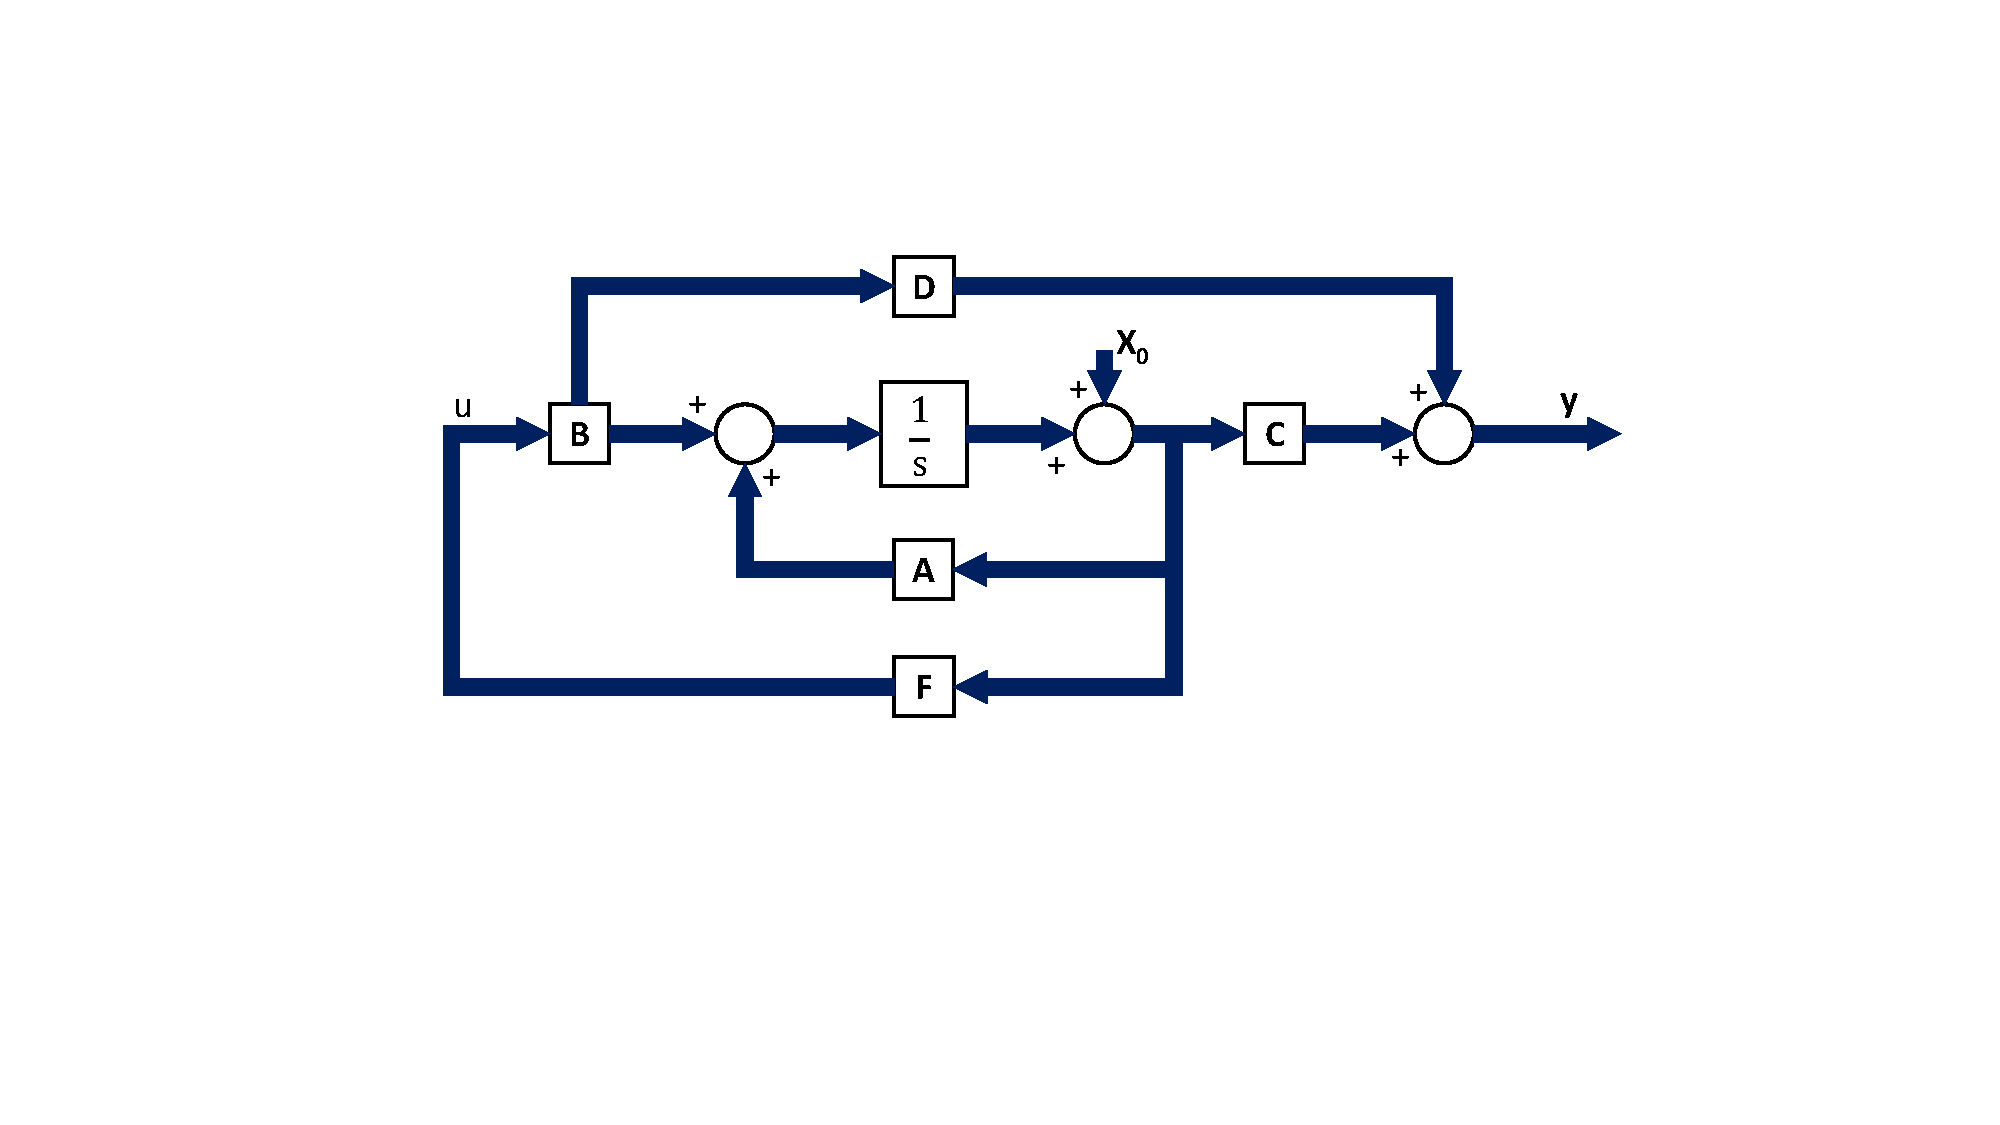
\includegraphics[width=\linewidth, trim={0 6.5cm 0 3.5cm}, clip]{Regelkreis}
\caption{Blockschaltbild Regelkreis, Quelle: eigene Darstellung, Inhalt aus \cite{RT2}}
\end{figure}

Die Stellgröße $u$ wird von einem Mikrokontroller mit einer Abtatsperiod $T_a = 20ms$ berechnet. Folglich handelt es sich um eine digitale Regelung. Um das Verhalten des diskreten Systems zu beschreiben müssen die diskreten Systemmatrizen $\textbf{A}_d$, $\textbf{B}_d$, $\textbf{C}_d$ und $\textbf{D}_d$ berechnet werden. Hierfür gilt nach \cite{RT2}:

\begin{equation}
\textbf{S} = T_a \sum_{v=0}^{\infty} \textbf{A}^v \frac{T^v}{(v+1)!}
\end{equation}
\begin{equation}
\textbf{A}_d = \textbf{I} + \textbf{S} \cdot \textbf{A}
\end{equation}
\begin{equation}
\textbf{B}_d = \textbf{S} \cdot \textbf{B}
\end{equation}
\begin{equation}
\textbf{C}_d = \textbf{C}
\end{equation}
\begin{equation}
\textbf{D}_d = \textbf{D}
\end{equation}

Die Reglermatrix $\textbf{F}$ wird als optimaler Zustandsregler nach dem quadratischen Gütekriterium entworfen. Die diskrete Gütefunktion für dieses System lautet:

\begin{equation}
\label{costfunction_equation}
I = \sum_{k=1}^\infty \textbf{x}^T(k) \cdot \textbf{Q} \cdot \textbf{x}(k) + R\cdot u(k)^2
\end{equation}

Die Matrizen $\textbf{Q}$ und $\textbf{R}$ stellen Gewichtungen der Zustands- und Stellgrößen dar. Die Ausgangswerte dieser Matrizen werden mit der Faustformel nach (\cite{lqrnotes}) berechnet. Ggf. können die Werte anschließend angepasst werden um die Reglergüte weiter zu verbessern.

\begin{equation}
\textbf{Q} = \begin{pmatrix}
\frac{1}{(\varphi_{max})^2} & 0 & 0 \\
0 & \frac{1}{(\dot{\varphi}_{max})^2} & 0 \\
0 & 0 & \frac{1}{(\dot{\psi}_{max})^2} \\
\end{pmatrix}
\end{equation}
\begin{equation}
R = \begin{pmatrix}
\frac{1}{(T_{M,max})^2}
\end{pmatrix}
\end{equation}

Die Reglermatrix $\textbf{F}$ muss die Eigenschaft besitzen die Gütefunktion (\ref{costfunction_equation}) zu minimieren. Dieses Problem wird mit Hilfe von der Matlab-Funktion \textit{lqrd} numerisch gelöst.

\subsubsection{Verifizierung des Reglers an dem 1D-Prototyp}
Mit Hilfe von Matlab wurden die Werte der Reglermatrix $\boldsymbol{F}$ berechnet.

\begin{equation}
\boldsymbol{F} = \begin{pmatrix}
0.8821 & 0.1386 & 0.0002
\end{pmatrix}
\end{equation}

Somit lässt sich das Motormoment $T_{M,n}$ durch die Rückführung des Zustandvektors $\boldsymbol{x}_n$ über die Reglermatrix $\boldsymbol{F}$ berechnen.

\begin{equation}
T_{M,n} = \boldsymbol{F} \cdot \boldsymbol{x}_n
\end{equation}

Der Regler wird zuerst mit Hilfe eines Simulink-Modelles in der Simulation überprüft. Anschließend wird der geschlossene Regelkreis auf den Prototyp übertragen. Hierbei ist zu beachten, dass bei der Modellierung des Systemverhaltens die Annahme getroffen wurde, dass der Schwerpunkt des Systems auf dessen Y-Achse liegt. Durch den unsymmetrischen Aufbau ist dies allerdings nicht der Fall, somit ergibt sich das folgende Gravitationsmoment  $M_G$, wobei der Winkel $\varphi_{cog}$ den Winkel zwischen Y-Achse und Schwerpunkt der Würfelseite bezeichnet.

\begin{equation}
M_G = g(m_K \cdot l_{AC} + m_R \cdot l_{AB}) \cdot sin(\varphi + \varphi_{cog})
\end{equation}

Somit muss ein konstantes Motormoment erzeugt werden, um die Würfelseite bei dem Sollwinkel $\varphi = 0$ zu halten. Dadurch wird die Schwungmasse konstant beschleunigt, weshalb die Schwungmasse nicht vollständig zum Stillstand kommen kann. Deshalb muss für die Berechnung des Drehmomentes der Winkel $\varphi_{cog}$ zu der Zustandsgröße $\varphi$ addiert werden.

\begin{equation}
T_{M,n} = \boldsymbol{F} \cdot \begin{pmatrix}
\varphi + \varphi_{cog} \\
\dot{\varphi} \\
\dot{\psi}
\end{pmatrix}
\end{equation}

Da die Winkelgeschwindigkeit der Schwungmasse $\dot{\psi}$ nur dann verschwindet wenn das Motormoment gleich null ist, kann der Wert von $\varphi_{cog}$ empirisch ermittelt werden.

Die folgenden Abbildungen zeigen den Verlauf der Winkelgeschwindigkeiten $\dot{\varphi}$ und $\dot{\psi}$. Hier zeigt sich, dass die Radgeschwindigkeit $\dot{\psi}$ nicht gegen null konvergiert. Mögliche Ursachen für dieses Verhalten sind neben der unsymmetrischen Konstruktion, die ungefilterten Werte von $\dot{\varphi}$ und $\dot{\psi}$, da deren Rauschsignale die Regelung negativ beeinflussen. Weiter können systematische Messabweichungen der Zustandsgrößen zu einer nicht verschwindenden Winkelgeschwindigkeit $\dot{\psi}$ führen.

\begin{figure}[h]
\centering
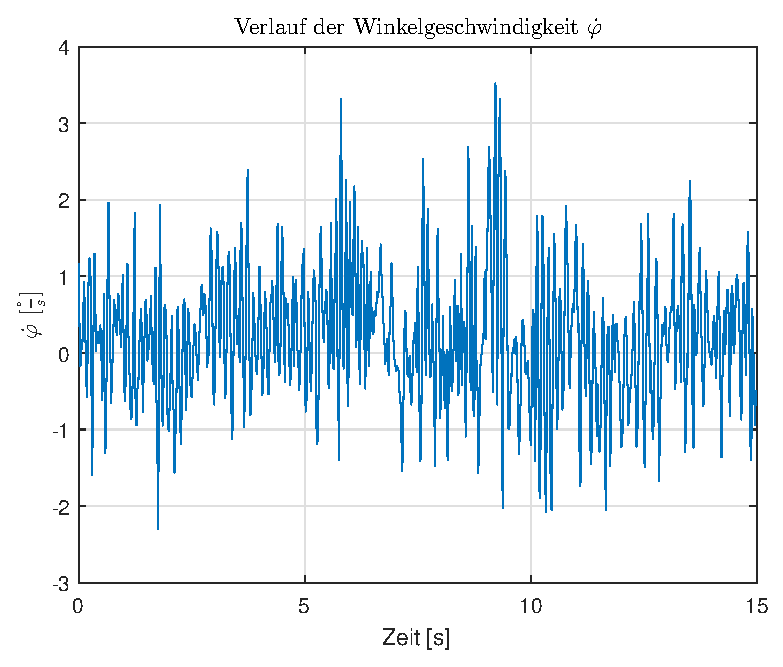
\includegraphics[scale=0.5]{img/phi__d_regelung}
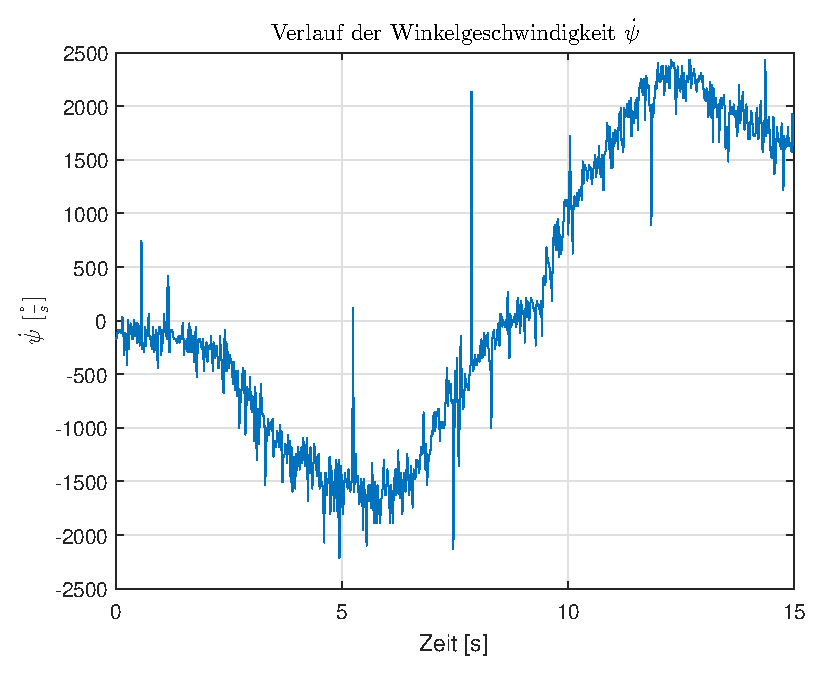
\includegraphics[scale=0.5]{img/psi__d_regelung}
\caption{Verluaf von $\dot{\varphi}$ und $\dot{\psi}$, Quelle: eigene Darstellung}
\end{figure}

\newpage
Die nächste Abbildung zeigt den Verlauf des Winkels $\varphi$, wobei die Werte der Winkelschätzung, des Komplementärfilters und des Kalman-Filters aufgezeigt sind. Hier lässt sich deutlich erkennen wie stark das rauschbehaftetes Signal der Winkelschätzung durch die jeweiligen Filter geglättet wird. Ein direkter Vergleich der beiden Filter ist ohne ein absolutes Referenzsignal nur schwer möglich.

\begin{figure}[h!]
\centering
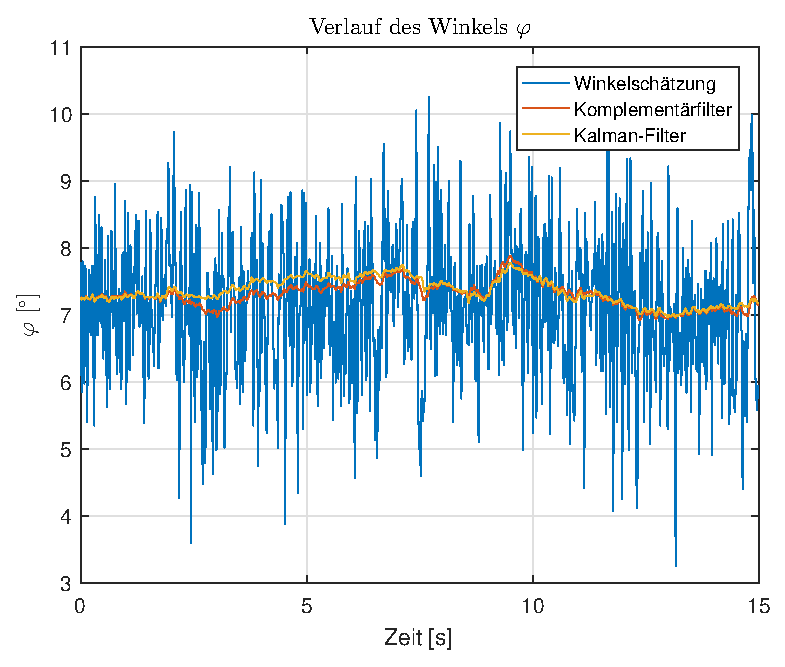
\includegraphics[width=0.5\linewidth]{img/phi_regelung}
\caption{Verlauf von $\varphi$, Quelle: eigene Darstellung}
\end{figure}

